\subsection{Package sequenziatore::client::imodel}
\begin{figure}[H] \centering 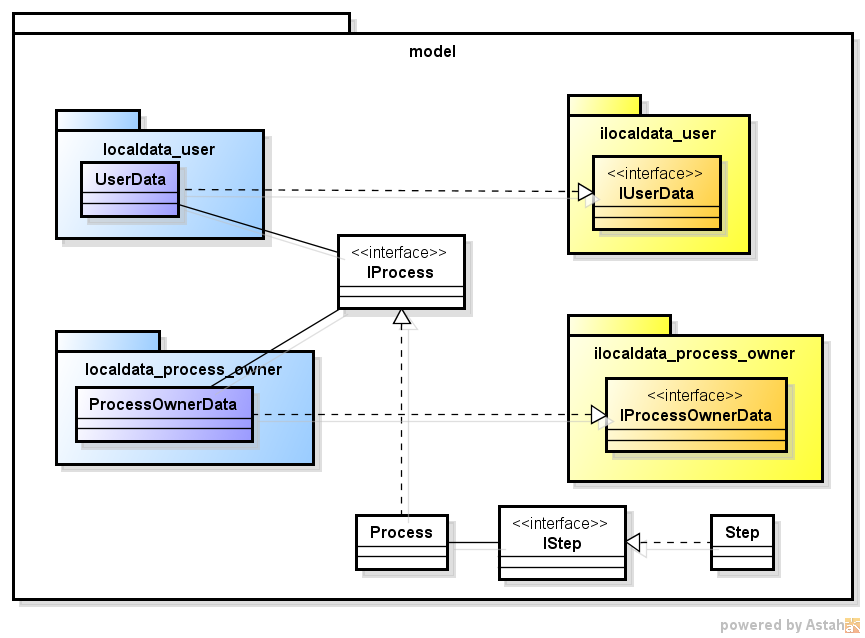
\includegraphics[width=%
\textwidth]
{./pack/clientmodel.png} \caption{Diagramma model del client}
\end{figure}
\subsubsection{Package sequenziatore::client::imodel::iprocessowner}
\paragraph{IProcessOwnerData}
\begin{itemize}
\item \textbf{Nome:} \texttt{IProcessOwnerData};
\item \textbf{Package:} \texttt{\iModelAdmin{}};
\item \textbf{Descrizione:} Interfaccia che permette di gestire i dati di un processo e il salvataggio in locale di tali dati.
\end{itemize}

\subsubsection{Package sequenziatore::client::imodel::iuser}
\paragraph{IUserData}
\begin{itemize}
\item \textbf{Nome:} \texttt{IUserData};
\item \textbf{Package:} \texttt{\iModelUser{}};
\item \textbf{Descrizione:} Interfaccia che permette di gestire i dati di un processo e il salvataggio in locale di tali dati.
\end{itemize}

\subsection{Package sequenziatore::client::model}
\subsubsection{Package sequenziatore::client::model}
\paragraph{IProcess}
\begin{itemize}
\item \textbf{Nome:} \texttt{IProcess};
\item \textbf{Package:} \texttt{\model{}};
\item \textbf{Descrizione:} Interfaccia che permette di gestire i dati di un processo.
\end{itemize}

\paragraph{IStep}
\begin{itemize}
\item \textbf{Nome:} \texttt{IStep};
\item \textbf{Package:} \texttt{\model{}};
\item \textbf{Descrizione:} Interfaccia che permette di gestire i dati di un passo di un processo.
\end{itemize}

\paragraph{Process}
\begin{flushleft}
\begin{itemize}
\item \textbf{Nome:} \texttt{Process};
\item \textbf{Package:} \texttt{\model{}};
\item \textbf{Descrizione:} Classe che permette di gestire i dati di un processo;
\item \textbf{Relazioni con altri componenti:}
\begin{sloppypar}
La classe implementa l'interfaccia \texttt{\model{}::I\fshyp{}Pro\fshyp{}cess} e utilizza oggetti di tipo \texttt{\model{}}::Step.
\end{sloppypar}
\end{itemize}
\end{flushleft}

\paragraph{Step}
\begin{flushleft}
\begin{itemize}
\item \textbf{Nome:} \texttt{Step};
\item \textbf{Package:} \texttt{\model{}};
\item \textbf{Descrizione:} Classe che permette di gestire i dati di un passo;
\item \textbf{Relazioni con altri componenti:}
\begin{sloppypar}
La classe implementa l'interfaccia \texttt{\model{}::I\fshyp{}Step}.
\end{sloppypar}
\end{itemize}
\end{flushleft}

\subsubsection{Package sequenziatore::client::model:processowner}
\paragraph{ProcessOwnerData}
\begin{flushleft}
\begin{itemize}
\item \textbf{Nome:} \texttt{ProcessOwnerData};
\item \textbf{Package:} \texttt{\modelAdmin{}};
\item \textbf{Descrizione:} Classe che permette di gestire i dati di un processo e il salvataggio in locale di tali dati;
\item \textbf{Relazioni con altri componenti:}
\begin{sloppypar}
La classe implementa l'interfaccia \texttt{\iModelAdmin{}::I\fshyp{}Pro\fshyp{}cess\fshyp{}Ow\fshyp{}ner\fshyp{}Da\fshyp{}ta} e utilizza oggetti di tipo \texttt{\model{}}::Pro\fshyp{}cess.
\end{sloppypar}
\end{itemize}
\end{flushleft}

\subsubsection{Package sequenziatore::client::model:user}
\paragraph{UserData}
\begin{flushleft}
\begin{itemize}
\item \textbf{Nome:} \texttt{UserData};
\item \textbf{Package:} \texttt{\modelUser{}};
\item \textbf{Descrizione:} Classe che permette di gestire un processo e il salvataggio in locale di tali dati;
\item \textbf{Relazioni con altri componenti:}
\begin{sloppypar}
La classe implementa l'interfaccia \texttt{\iModelUser{}::I\fshyp{}U\fshyp{}ser\fshyp{}Da\fshyp{}ta} e utilizza oggetti di tipo \texttt{\model{}}::Pro\fshyp{}cess.
\end{sloppypar}
\end{itemize}
\end{flushleft}